\section{\textsc{Introduction}}
\hrule height 0.5pt
\vspace*{2.5pt}
Traditionally, the primary technique used in developing terrain has been handcraft,
using modelling software to precisely describe the creations. However, this approach
suffers from four main drawbacks (Roden \& Parberry, 2004):
\begin{itemize}
    \item \textbf{Operability:} handcrafted terrains are slow and resource-intensive, requiring
    manual adjustments for every detail.
    \item \textbf{Inflexibility:} modifying completed designs can dramatically alter technical
    requirements.
    \item \textbf{Incompatibility:} handcrafted terrains often lack coherence with physics engines
    and other computational models.
    \item \textbf{Unscalability:} as virtual worlds grow in complexity with their expansive, dynamic
    environment, handcrafted terrains become impractical.
\end{itemize}
In the late 1960s, computer graphics pioneers confronted these setbacks, seeking ways to simulate natural
patterns without the efficiencies of manual design (Autodesk, 2024). The answer manifested in the form of
\emph{\textbf{noise algorithms}}, mathematical functions capable of producing structured randomness, often termed ``pseudo-randomness''
(Perlin, 2001). Over the decades, they have evolved beyond gaming applications to enable hyper-realistic CGIs in films
(Pegg, 2010), creating texture (Perlin, 1985), and advancing fluid dynamics simulations (Kim et al., 2008). 

My fascination with noise algorithms began in the blocky worlds of the game Minecraft. As a teenager, I spent countless
hours exploring its vast biomes, awestruck by the seamless blend of towering cliffs, dense forests, and sprawling cave systems.
While I appreciate the aesthetics of the game, I lacked insight into the technical requirements underpinning it. Years later, I 
discovered the role of noise in shaping these landscapes and became curious about which aspects of noise contribute to terrain realism. 
\begin{figure}[H]
    \centering
    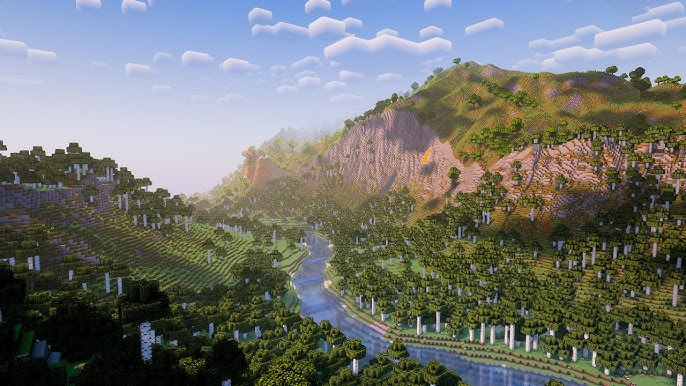
\includegraphics[width=0.32\textwidth]{minecraft1.jpg}
    \includegraphics[width=0.32\textwidth]{minecraft3.png}
    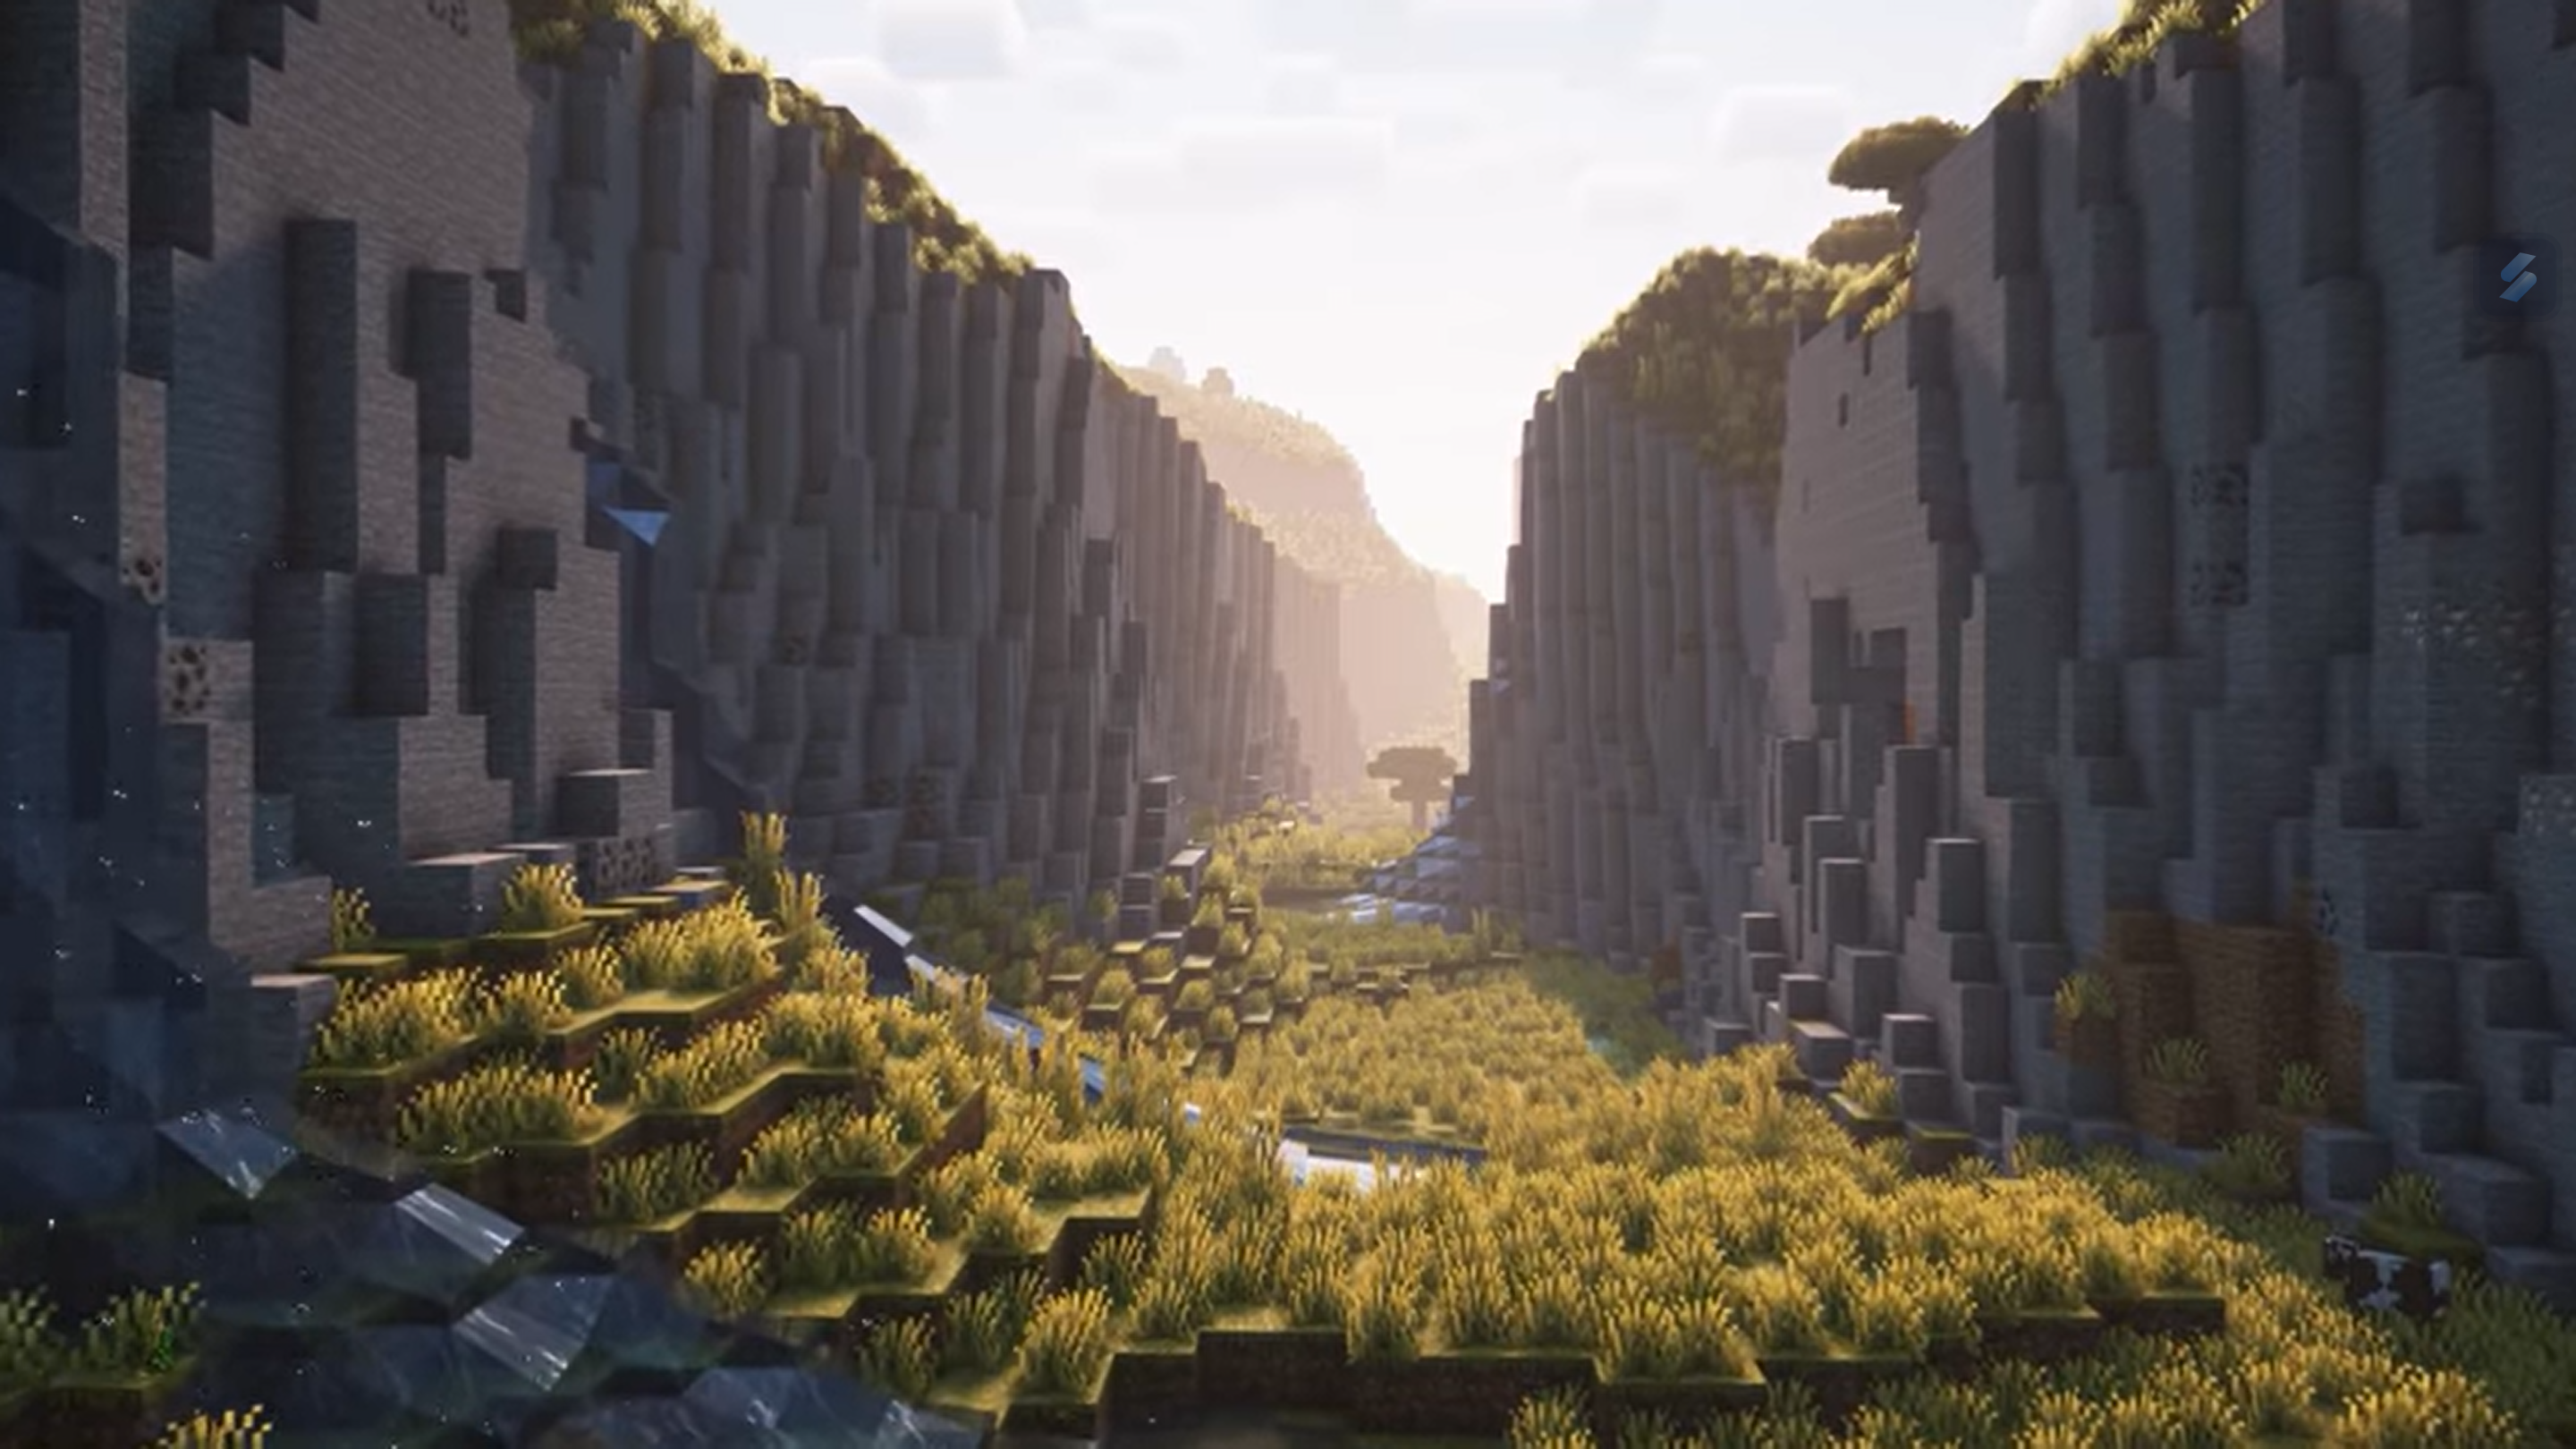
\includegraphics[width=0.32\textwidth]{minecraft4.png}
    \includegraphics[width=0.32\textwidth]{minecraft5.png}
    \includegraphics[width=0.32\textwidth]{minecraft6.png}
    \includegraphics[width=0.32\textwidth]{minecraft7.png}
    \caption{Minecraft terrains generated with noise functions. Images retrieved from (iambeen, 2022)}
    \label{fig:minecraft}
\end{figure}
There are two main types of noise commonly used in terrain generation (Figure \ref{fig:noise_intro}): Value noise and Perlin noise. Value noise generates random values at fixed grid points 
and uses interpolation to smoothly transition between them. Perlin noise, on the contrary, assigns gradient vectors (directions) at grid points and computes the 
dot product between the gradient vector and relative position vectors, leading to smoother transition and more natural gradients. Despite their popularity, there 
has been very little rigorous academic research directly comparing their ability to replicate real-world terrain, thus this investigation involves a degree of 
personal risk-taking in exploring largely uncharted territory. 
The aim of this IA is to determine which algorithm, Value noise or Perlin noise, generates terrain with statistical distribution more closely resembling
real-world elevation data. To evaluate this, the following metrics will be used:
\begin{itemize}
    \item Elevation distribution using \textbf{Histograms of normalised height values} and other \textbf{Statistical moments}, such as mean, variance, kurtosis, to measure how terrain heights are spread out across the map.
    \item Spatial autocorrelation using \textbf{Moran's I} to measure global clustering trends.
    \item Spectral characteristics using \textbf{Power Spectral Density} to break down how much terrain variation occurs at different spatial scales.
\end{itemize}
These properties will be benchmarked against elevation data from the Global Multi-resolution Terrain Elevation Data (GMTED2010), a model developed through a
collaborative effort between the U.S. Geological Survey (USGS) and the National Geospatial-Intelligence Agency (NGA). 

\begin{figure}[H]
    \centering
    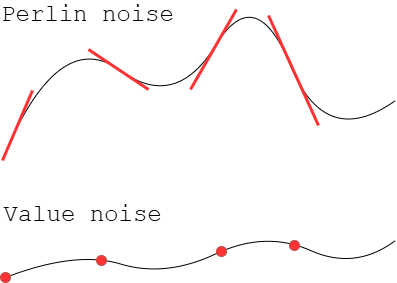
\includegraphics[width=0.5\textwidth]{noise intro.png}
    \caption{Simplified representation of Value and Perlin noise}
    \label{fig:noise_intro}
\end{figure}

Terrain maps will be generated on a fixed $256\times256$ grid with normalised height values $z\in[0,1]$. Both algorithms are tested
under identical spectral parameters, including amplitude, frequency, persistence, lacunarity, and number of octaves. To ensure smooth transitions 
in terrain and avoid visible artifacts, a cubic smoothstep interpolation is applied when blending values between grid points. This is a type of 
interpolation where the function's slope is zero at both endpoints, producing a smooth and continuous curve that avoids sharp changes. A fixed seed 
($30042603$) will be employed to ensure deterministic comparisons by removing the randomness of the height values out of the effects. Python will 
be used for all implementations, with the complete code included in the Appendix.

Based on prior literature and the mathematical formulation of each algorithm, I predict that Perlin noise will more closely match the spatial 
autocorrelation and spectral characteristics of real terrain due to its gradient-based interpolation, which tends to produce smoother, more 
coherent structures. On the other hand, Value noise, may better approximate the elevation distribution, especially if carefully tuned, but is 
expected to perform worse on large-scale spatial patterns due to its reliance on value interpolation.